\documentclass[10pt,a4paper]{amsart}

\usepackage[]{graphicx}
\usepackage[]{hyperref}
\usepackage[]{physics}
\usepackage[]{listings}
\usepackage[utf8]{inputenc}
\usepackage[toc,page]{appendix}
\usepackage[dvipsnames]{xcolor}
\usepackage{tikz}


\definecolor{mygray}{gray}{0.9}

\lstset{
	frame = single,
	language = C++,
	showstringspaces = false,
	tabsize = 2,
	otherkeywords = {self},
	keywordstyle = \color{Maroon},
	identifierstyle=\color{olive},
 	stringstyle=\color{orange},
 	backgroundcolor=\color{mygray},
 	breaklines = true
}

\title[Ising Model]{The Ising model and the Metropolis Algorithm \\ 
	\hrulefill\small{ FYS3150: Computational Physics }\hrulefill}
	
\author[Winther-Larsen]{Sebastian G. Winther-Larsen \\
\href{https://github.com/gregwinther/FYS3150/}{\texttt{github.com/gregwinther}}}
	
\date{\today}

\begin{document}

\begin{titlepage}
\begin{abstract}
The aim of this project is to determine the Curie temperature $T_c$, of a system undergoing phase transitions. When the temperature is raised above this critical level a ferromagnetic material will change into a paramagnetic material. The aim is to solve the problem employing the Metropolis-Hastings algorithm and Monte Carlo methods.
\end{abstract}
\maketitle
\tableofcontents
\end{titlepage}

\section{Introduction}
This study is both an exercise in the use of Monte Carlo methods and an analysis of the very popular Ising model. Monte Carlo methods are applicable in several situations where many other methods are too computationally heavy. They are a broad class of methods that rely on random sampling to obtain numerical results. The Ising model is a mathematical model of ferromagnetism in statistical mechanics. The Ising model and Monte Carlo methods go hand in hand as we shall see in this study.

I will start by giving a very brief description and definition of the two-dimensional Ising model. This general model will be simplified by assuming zero extern field which leads to a simple energy equation. Then I will present the Metropolis-Hastings algorithm and how it is implemented using Monte Carlo methods. Lastly, several simulations are presented, and I will try to uncover the Curie temperature where the ferromagnetic model transitions into a paramagnetic one.

\section{Theory}
The model we will employ in this study of phase transitions at finite temperature for magnetic systems is the Ising model, named after Ernst Ising who solved a one-dimensional variant of the model\cite{Ising}. The two-dimensional square lattice model, employed herein, was given an analytic description much later by Lars Onsager\cite{Onsager}.

\subsection{The general Ising model}
Let $\Lambda$ be a set of lattice positions, each with adjacent positions, forming a $d$-dimensional lattice. For each lattice site, $k \in \Lambda$, there is a discrete variable $\sigma_k \in \{+1,-1\}$, representing the spin of the site, $\uparrow$ and $\downarrow$, respectively. A spin configuration $\sigma$ is a specific spin configuration of the lattice.

For two adjacent sites, $i,j \in \Lambda$, one has an interaction $J_{ij}$. A site $j \in \Lambda$ will also have an external magnetic field $h_j$ interacting with it. The energy of a specific system is given by the following Hamiltonian
\begin{equation}
\label{eq:IsingHamilton}
E = H(\sigma)= -\sum_{\ev{ik}}J_{ij}\sigma_i \sigma_j - \mu \sum_j h_j \sigma_j,
\end{equation}
where the first sum is over pairs of adjacent spins. The notation $\ev{ij}$ indicates that sites $i$ and $j$ are nearest neighbours. In the second sum, $\mu$ is the magnetic moment.

The probability of a certain configurations is given by the Boltzmann distribution
\begin{equation}
\label{eq:Boltzmann}
P_\beta(\sigma) = \frac{e^{-\beta H(\sigma)}}{Z_\beta}
\end{equation}
where $Z_\beta$ is the partition function acting as a normalisation constant, and $\beta=(k_BT)^{-1}$. This would mean that by increasing the temperature $T$, finding the system in one particular configuration decreases. It must be so, because with a relatively higher temperature, one would expect previously unfavourable configuration to become more feasible.

There are two important expected values that are important in order to characterise a magnetic system. The \emph{mean energy} of the system is
\begin{equation}
\label{eq:meanenergy}
\ev{E} = \sum_{i=1}^ME_iP_\beta(\sigma) = \frac{1}{Z}\sum_{i=1}^ME_ie^{-\beta E_i},
\end{equation}
and the \emph{mean magnetisation} is
\begin{equation}
\label{eq:meanmagnet}
\ev{\mathcal{M}} = \sum_{i=1}^M\mathcal{M}_iP_\beta(\sigma) = \frac{1}{Z}\sum_{i=1}^M\mathcal{M}_ie^{\beta E_i},
\end{equation}
where $\mathcal{M}_i = \sum_{j \in \Lambda}\sigma_j$ for all configurations $\sigma$, and $M$ denotes the number of possible configurations. Another quantity of interest is \emph{magnetic susceptibility} $\chi$ which tells us how much an extensive parameter changes when an intensive parameter increases. It is given by
\begin{equation}
\label{eq:susceptibility}
\chi = \frac{1}{k_BT}(\ev{\mathcal{M}^2} - \ev{\mathcal{M}}^2).
\end{equation}
The \emph{heat capacity}, at constant volume, is given by
\begin{equation}
\label{eq:heatcap}
C_V = \frac{1}{k_BT^2}(\ev{E^2}-\ev{E}^2)
\end{equation}

The minus sign on each term of the Hamiltonian $H(\sigma)$ in equation \ref{eq:IsingHamilton} is conventional. By this sign convention, the Ising model can be classified according to the sign of the interaction. If, for all pairs $i,j$:
\begin{itemize}
\item $J_{ij} > 0$, the interaction is ferromagnetic,
\item $J_{ij} < 0$, the interaction is anti-ferromagnetic,
\item $J_{ij} = 0$, the spins are non-interacting.
\end{itemize}
In a ferromagnetic Ising model, spins desire to be aligned: the configurations in which adjacent spins are of the same sign have higher probability. In an anti-ferromagnetic model, adjacent spins tend to have opposite signs.

\subsection{Simplified ferromagnetic Ising model}
The general Ising model, as described above, will not be used in this study, but a much simpler version of it. Firstly, we will examine a system with no external magnetic field, as was originally solved analytically by Onsager\cite{Onsager}. Because the second sum in the Hamiltonian in equation \ref{eq:IsingHamilton} is zero, and we are left with
\begin{equation}
\label{eq:IsingHamSimple1}
E = H(\sigma) = -\sum_{\ev{ik}}J_{ij}\sigma_i\sigma_j.
\end{equation} 
Secondly, we assume that the coupling constant $J_{ij}$, that describe the interaction of a spin with its neighbour, to be constant. That is $J_{ij} = J \forall i,j \in \Lambda$ and equation \ref{eq:IsingHamSimple1} is simplified further to
\begin{equation}
\label{eq:IsingHamSimple2}
E = H(\sigma) = -J \sum_{\ev{ik}}\sigma_i\sigma_j
\end{equation}

In this study, we will assume that we have a ferromagnetic ordering, id est  $J>0$. This means that neighbouring spins are aligned, because it would lead to lower energy. It is easy to see why it must be so, as $\sigma_i\sigma_j=1$ whenever spin $i$ and $j$ have the same sign.

\subsection{Example: $2\times2$ Ising model}
It would be beneficial to test the waters of the ocean of the vast ocean that is the Ising model, by a two-dimensional model with lattice dimension $L=2$ and periodic boundary conditions. This model has $s=2^4=16.$ different configurations $\sigma$. The energy of a given configuration would be
\begin{equation*}
E_i = -J \sum_{\ev{kl}}^4 \sigma_k \sigma_l.
\end{equation*}

Figure \ref{fig:2by2lattice} shows an arbitrary configuration of a $2\times2$ spin lattice. The energy for this configuration is
\begin{equation*}
E_i = -J((+1)(-1)+(+1)(-1)+(+1)(-1)+(+1)(-1)) = 8J
\end{equation*}
which happens to be the highest energy possible for the system. When all spins are parallel we see that $E_i=-8J$ which is the lowest energy possible. If only one spin would differ from the others, the energy would be $E_i = 0$ and so on. Of the $16$ possible configurations, several will have degeneracies ($\Omega(E_i)$), which corresponds to the number of configurations with the same energy. Moreover, the magnetisation of a particular configuration is simply the sum of the spins and is easy to calculate. All the possible configurations of this system can be found in table \ref{tab:2by2lattice}.

\begin{figure}[h]
	\centering
	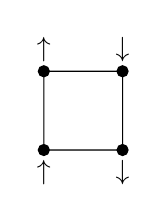
\begin{tikzpicture}
	\filldraw 	(0,0) circle(2pt) node[align=left, below]{$\uparrow$}-- 
				(0,1) circle(2pt) node[align=left, above]{$\uparrow$}-- 
				(1,1) circle(2pt) node[align=right, above]{$\downarrow$}-- 
				(1,0) circle(2pt) node[align=right, below]{$\downarrow$}-- (0,0);
	\end{tikzpicture}
	\caption{Sample $2\times2$ spin lattice.}
	\label{fig:2by2lattice}
\end{figure}

\begin{table}
	\centering
	\caption{All possible configurations of a $2\times2$ Ising model}
	\begin{tabular}{cccc} \hline
	No of $\uparrow$ & $\Omega(E_i)$ & $E_i$ & $\mathcal{M}_i$ \\ \hline
	$4$ & $1$ & $-8J$ & $4$  \\
	$3$ & $4$ & $0$   & $2$ \\
	$2$ & $4$ & $0$   & $0$  \\
	$2$ & $2$ & $8J$  & $0$  \\
	$1$ & $4$ & $0$   & $-2$ \\
	$0$ & $1$ & $-8J$ & $-4$ \\ \hline
	\end{tabular}
	\label{tab:2by2lattice}
\end{table}

Now to compute the physical quantities as discussed above, expected value for energy $\ev{E}$, expected value for magnetisation $\ev{\mathcal{M}}$, expected value for specific heat $\ev{C_V}$, and susceptibility $\chi$. For the $2\times2$ Ising model these quantities have closed form expressions. The partition function for the system is given by
\begin{equation}
\label{2by2partition}
Z = \sum_{i=1}^16 e^{-\beta E_i} = e^{\beta8J} + 12 + 2e^{-\beta8J} + e^{\beta8J} = 4\cosh(\beta8J) + 12
\end{equation}
The expected energy is
\begin{equation}
\label{2by2expectedE}
\ev{E} = -\frac{\partial}{\partial\beta} \ln Z = -\frac{\partial}{\partial \beta}\ln(4\cosh(\beta J) + 12)
 = -8J \frac{\sinh(8\beta J)}{\cosh(8\beta J) + 3}.
\end{equation}
The mean magnetisation for this system is easiest to compute with equation \ref{eq:meanmagnet}, merely adding all possible states and dividing by the partition function.
\begin{equation}
\label{eq:2by2meanmagnet}
\ev{\mathcal{M}}= \frac{1}{Z}(-4e^{8\beta J} - 8e^0 + 8e^0 +8e^{8\beta J}) = 0
\end{equation}
the expected absolute magnetisation, on the other hand, becomes
\begin{equation}
\label{eq:2by2absmeanmagnet}
\ev{\abs{\mathcal{M}}} = \frac{1}{Z}(4e^{8\beta J} + 8e^0 + 8e^0 + 4e^{8\beta J}) = \frac{4 +2 e^{8\beta J}}{\cosh(8\beta J) +3}.
\end{equation}
The expected value for specific heat is
\begin{equation}
\label{eq:2by2specificheat}
\ev{C_V} = \frac{1}{k_bT^2}\frac{\partial^2}{\partial\beta^2}
\end{equation}
inserting equation \ref{2by2expectedE} gives
\begin{align*}
\ev{C_V} 	&= -\frac{1}{k_BT^2}\frac{\partial}{\partial\beta}\left(-8J\frac{\sinh(8\beta J)}{\cosh(8\beta J)+3} \right) \\
			&= \frac{1}{k_BT^2}\left(\frac{64J^2\cosh(8\beta J)}{\cosh(8\beta J)+3}-\frac{64J^2\sinh^2(8\beta J)}{(\cosh(8\beta J)+3)^2}\right) \\
			&= \frac{1}{k_BT^2}\frac{64J^2}{\cosh(8\beta J) + 3}\left(\cosh(8\beta J) - \frac{\sinh^2(8\beta J)}{\cosh(8\beta J) +3} \right)
\end{align*}

The susceptibility $\chi$ of a thermodynamic system is easy to compute if one knows what the variance of magnetisation, $\sigma_{\mathcal{M}}^2)$, is. Rewriting equation \ref{eq:susceptibility} gives
\begin{equation}
\label{eq:susceptibility2}
\chi = \frac{1}{k_BT}\sigma_{\mathcal{M}}^2.
\end{equation}
Using equations \ref{eq:2by2meanmagnet} and \ref{eq:2by2absmeanmagnet} one can deduce that the variance of the magnetisation must be
\begin{equation}
\label{eq:2by2magnetvar}
\sigma_{\mathcal{M}}^2 = \ev{\mathcal{M}^2} - \ev{\mathcal{M}}^2 = \frac{32}{Z}(e^{8\beta J} +1) - 0 = \frac{8(e^{8\beta J} + 1)}{\cosh(8\beta J) + 3}.
\end{equation}
Inserting \ref{eq:2by2magnetvar} into \ref{eq:susceptibility2} yields the susceptibility for the system
\begin{equation}
\label{eq:2by2susceptibility}
\chi = \frac{8(e^{8\beta J}+1)}{k_BT(\cosh(8\beta T) + 3)}
\end{equation}

Bear in mind that $\beta = \frac{1}{k_BT}$, and that all the quantities computed are functions of $T$. The results computed here can be used as comparison for numerical computations.

\section{Algorithm}
An initial spin configuration will be 

\subsection{Markov chains}
A Markov chain gives a good description for a system that moves towards a steady state given an initial configuration. A Markov process is a random walk with a a set of probabilities for making a set of moves. Such a process is usually represented by a stochastic matrix containing probabilities of transitioning from one state to another. In physics Markov chains can by used to study diffusion because it gives a framework for the rules of Brownian motion - the behaviour exhibited by small parts of any system when exposed to random fluctuations of the medium.

In order to simulate how the system in this study evolves towards a steady state, Markov chains are used repeatedly in Monte Carlo simulations. From Markov chains one gets tow conditions needed for reaching a steady state, detailed balance and ergodicity. These properties governs our choice of algorithm, the Metropolis-Hastings algorithm.

\subsection{The Metropolis-Hastings algorithm}
In this project we need random samples from a probability distribution $P_\beta (\sigma)$ associated with the physical system we wish to model. Regrettably, direct sampling can be incredibly difficult, as we need to compute the partition function in order to express the probability distribution in its entirety. The Metropolis-Hastings algorithm is circumvents this problem because it only requires a function $f$ proportional to the distribution density.

The Metropolis-Hastings algorithm can be condensed down to the following steps.
\begin{enumerate}
\item The system is initialised by an initial state which can be randomly generated. The energy $E_b$ of this configuration is computed.
\item The initial configuration is changed by flipping the spin of an arbitrary site. One then computes the energy of this new trial state $E_t$.
\item The difference in energy between the two states $\Delta E = E_t - E_b$ is calculated. For the two-dimensional Ising model there are only five different possilbe values for $\Delta E$.
\item If $ \Delta E < 0$ the new configuration is accepted, meaning that the energy is lower than it was, and the system is progressing towards an energy minimum.
\item If $ \Delta E > 0$ one computes $w = e^(\beta \Delta E)$ and compares $w$ to a random number $r$. If $r < w$ the state is accepted, else the inital state is kept.
\item The expectation values are updated. And the steps are repeated until a sufficiently good steady state is reached.
\end{enumerate}

As stated above, the possible different energy changes for a two-dimensional Ising model are finite. The possible changes are $\Delta E = 8J, 4J, 0, -4J, -8J$.  An array containing these values is constructed which contains the possible values before doing the Metropolis sampling. One can compare the possible energy changes against elements of this array instead of computing $w$ for every other iteration. This should vastly increase computing speed.

The algorithm determines whether a proposed move is implemented based on a transition probability and an acceptance probability. The strength of the algorithm is that the transition probability need not be known. 

\section{Implementation}
The Ising model is implemented in C++ in the class \lstinline|Ising.cpp| contains all the methods necessary for a simulation of the model. The full program with can be found by following the link at the front page of this article.

\subsection{Ising class}
An object-oriented approach was picked in order to increase flexibility and tidiness. The only data structure that exists outside the Ising class is the array of expected values, for easy comparison between several class instances. As the program is built right now, it can be run with command line arguments for spin lattice size, temperature domain and number of Monte Carlo cycles, which called $M$ times by \lstinline|simulate| adds up to a total complexity of $\mathcal{O}(ML^2)$.

Of the various methods incorporated in the \lstinline|Ising| class, \lstinline|simulate| and \lstinline|metropolis| are the most important ones. The method \lstinline|simulate| calls the \lstinline|metropolis| for every Monte Carlo cycle. Denoting $L$ as the spin lattice dimension and $M$ the number of Monte Carlo cycles, each call of \lstinline|metropolis| constitutes a complexity of $\mathcal{O}(L^2)$.

\section{Simulations}

\subsection{$2\times2$ Ising model with $T=1$}
Figure \ref{tab:2by2analMC} shows how increasing number of Monte Carlo cycles measures up to the analytic (exact) solution for a $2\times2$ system. One can see that it is necessary to have towards $1000000$ cycles in order to get the best estimates. This is an important results when making further computations. Moreover, a diagram of the magnetisation and energy of this system is shown in figure

\begin{table}
	\centering
	\caption{Comparison between Monte Carlo simulations at different length and the analytical solution for a $2\times2$ system.} \label{tab:2by2analMC}
	\begin{tabular}{lccccc} \hline
	$M$ & $\ev{E}$ & $C_V$ & $\chi$ & $\ev{\mathcal{M}}$ \\ \hline
	100         &  $-2$ & $0$ & $0$ & $1$ \\
	1000       & $-1.998$ & $0.015984$ & $0.03996$ & $0.6235$ \\
	10000     & $-1.9964$ & $0.028748$ & $0.003594$ & $0.44705$ \\
	100000   & $-1.99626$ & $0.029864$ & $0.003694$ & $0.040625$ \\
	1000000 & $-1.995968$ & $0.032191$ & $0.0039439$ & $0.059681$ \\ \hline
	Analytical & $ -1.99598 $ & $0.03208$ & $0.00401$ &  $0$ \\ \hline
	\end{tabular}
\end{table}

\begin{figure}
	\centering
	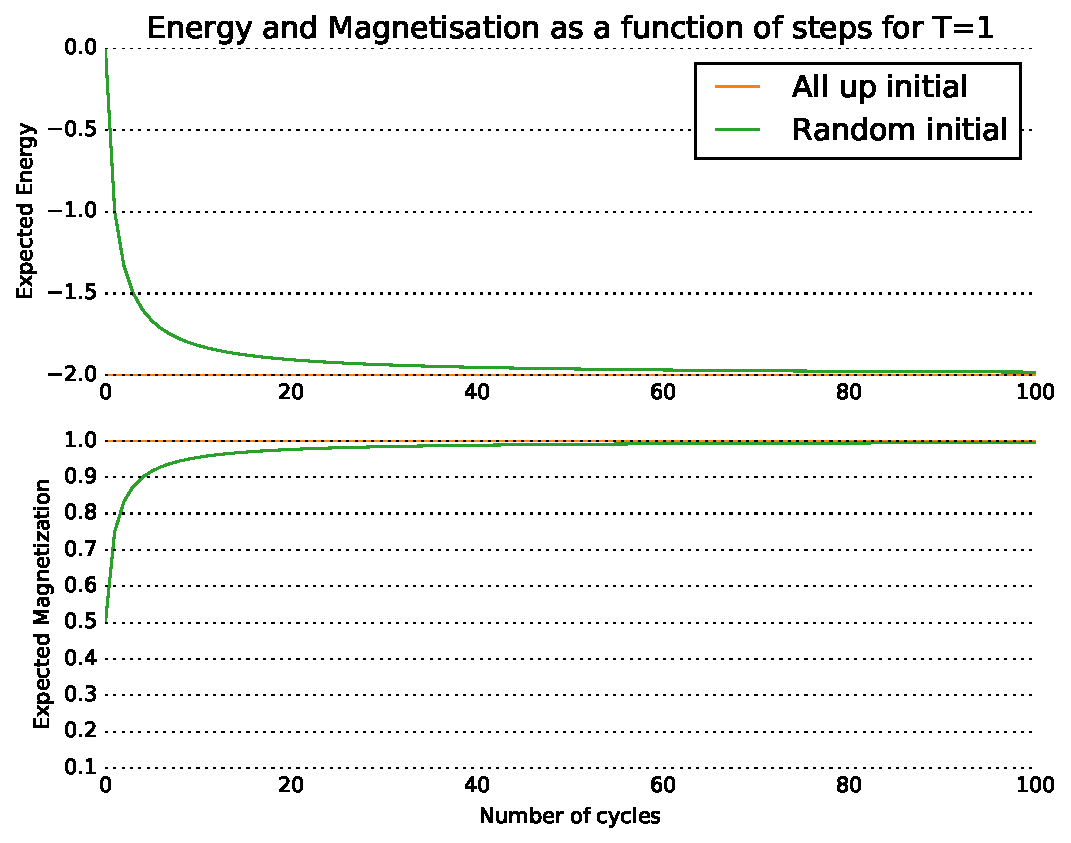
\includegraphics[width=0.9\textwidth]{../figures/EandM_2_T1_bothorient.pdf}
	\caption{Energy and Magnetisation as a function of Monte Carlo cycles for the $2\times2$ system. \label{fig:2by2simple}}
\end{figure}

\subsection{$20\times20$ Ising model}

We are interested in figuring out how many Monte Carlo cycles are necessary in order to establish an steady state. This must be done in order to know where it is alright to start calculation expected values. If we start the computations before a steady state is reached in the system, the results can be skewed.  How the system approaches a steady state can already be seen in figure \ref{fig:2by2simple}. In this figure though, a mere hundred Monte Carlo cycles were conducted, and the system is indeed incredibly small. Therefore, we consider both an initial random configuration for a larger $20 \times 20$ spin system, both for temperatures $T=1$ and $T=2.4$. The result of this simulation can be found in figure \ref{fig:temp1and2.4}. This simulations has been allowed to run for a one million Monte Carlo cycles. One can clearly see that both systems starts at some configuration which is some distance away from the equilibrium and then quickly falls (rises) asymptotically towards a steady state. Interestingly, for the higher temperature, magnetisation behaves differently than for the lower temperature. 

\begin{figure}
	\centering
	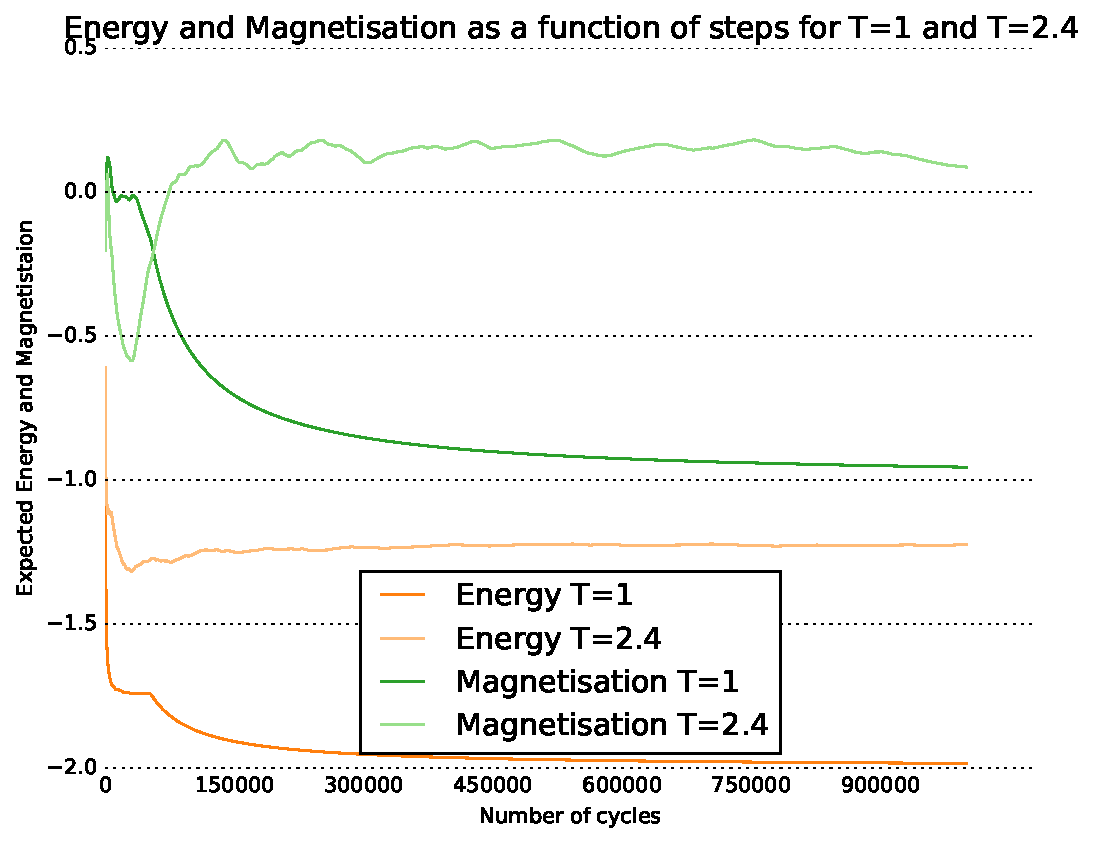
\includegraphics[width=0.9\textwidth]{../figures/20EandMT1and24.pdf}
	\caption{Mean Energy and Mean magnetisation for a $20 \times 20$ spin lattice with temperatures $T=1$ and $T=2.4$. \label{fig:temp1and2.4}}
\end{figure}

It would also be interesting to see how many spin changes of the Metropolis-Hastings algorithm are accepted at this higher temperature. A plot for accepted configuration changes as a function of cycles for the two temperatures $T=1$ and $T=2.4$ is shown in figure \ref{fig:acceptedstates}. One can clearly see that for the higher-temperature system the number of accepted states linearly proportional to the number of cycles in the simulation, while for the lower-temperature system the number of accepted states stay the same after the steady state is reached.  

\begin{figure}
	\centering
	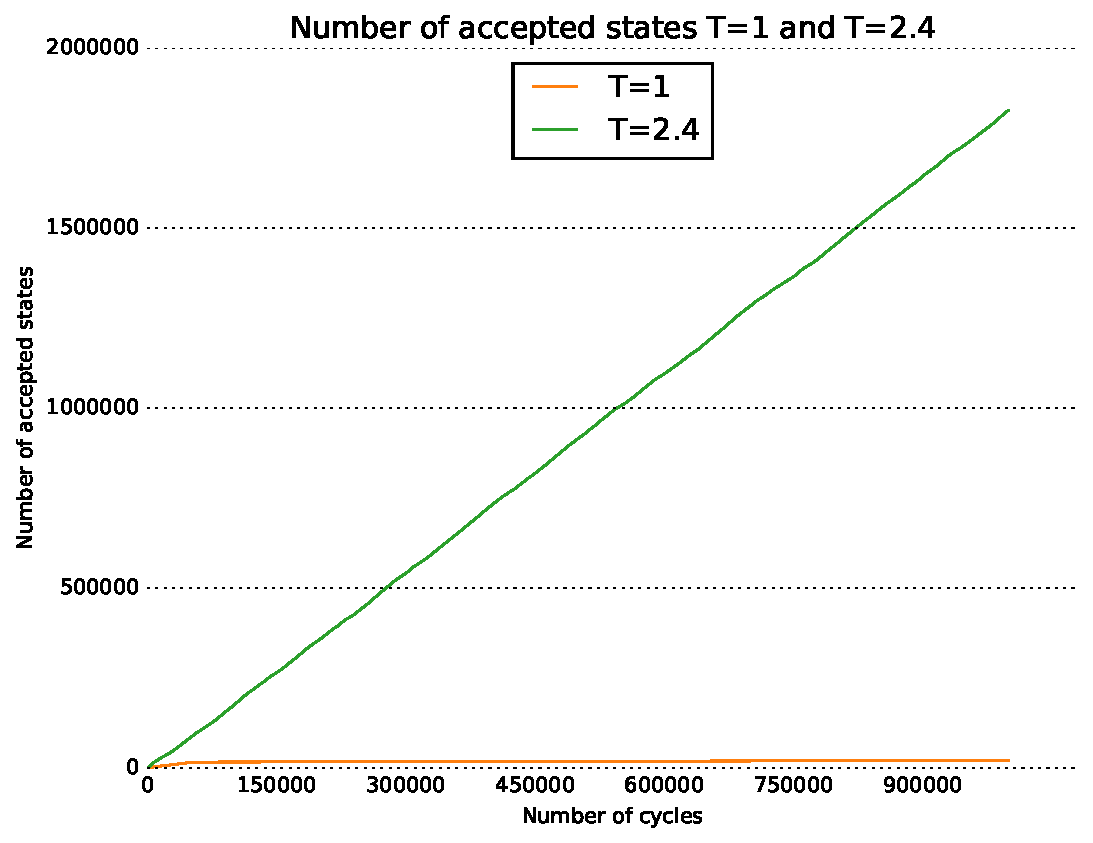
\includegraphics[width=0.9\textwidth]{../figures/20NaccofNT1and24.pdf}
	\caption{Figure showing that the number of accepted states for a higher-temperature system ($T=2.4$) rises linearly, while the accepted states for for a lower-temperature system ($T=1$) stays the constant at equilibrium.\label{fig:acceptedstates}}
\end{figure}

The probabilities for finding the system in a given configuration will also change for a higher temperature. A simulation of the probability density functions of the $20\times20$ system for temperatures $T=1$ and $T=2.4$ is given in figure \ref{fig:pde}. One can see that the probability for finding the system at a higher energy is moved larger at a higher temperature, as one would expect.

\begin{figure}
	\centering
	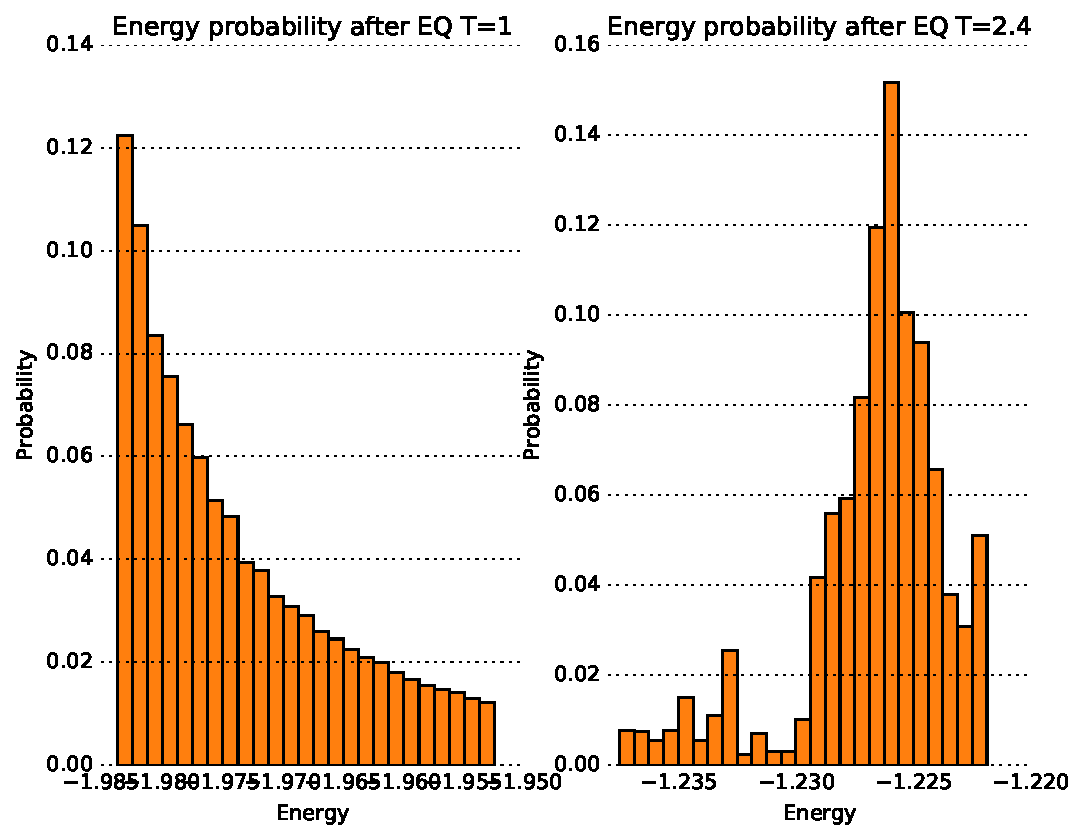
\includegraphics[width=0.9\textwidth]{../figures/EhistProbBothT.pdf}
	\caption{Probability densities for a lower temperature $T=1$ and a higher temperature $T=2.4$. \label{fig:pde}}
\end{figure}

\subsection{Larger spin lattices}

Figure \ref{fig:largersystems} depicts the expected energy $\ev{E}$, average absolute magnetisation $\ev{\abs{\mathcal{M}}}$, specific heat $C_V$ and susceptibility $\chi$ as functions of temperature $T \in [2.0,2.4]$ for large spin lattices $L=20$, $L=40$, $L=60$ and $L=80$.  

\begin{figure}
	\centering
	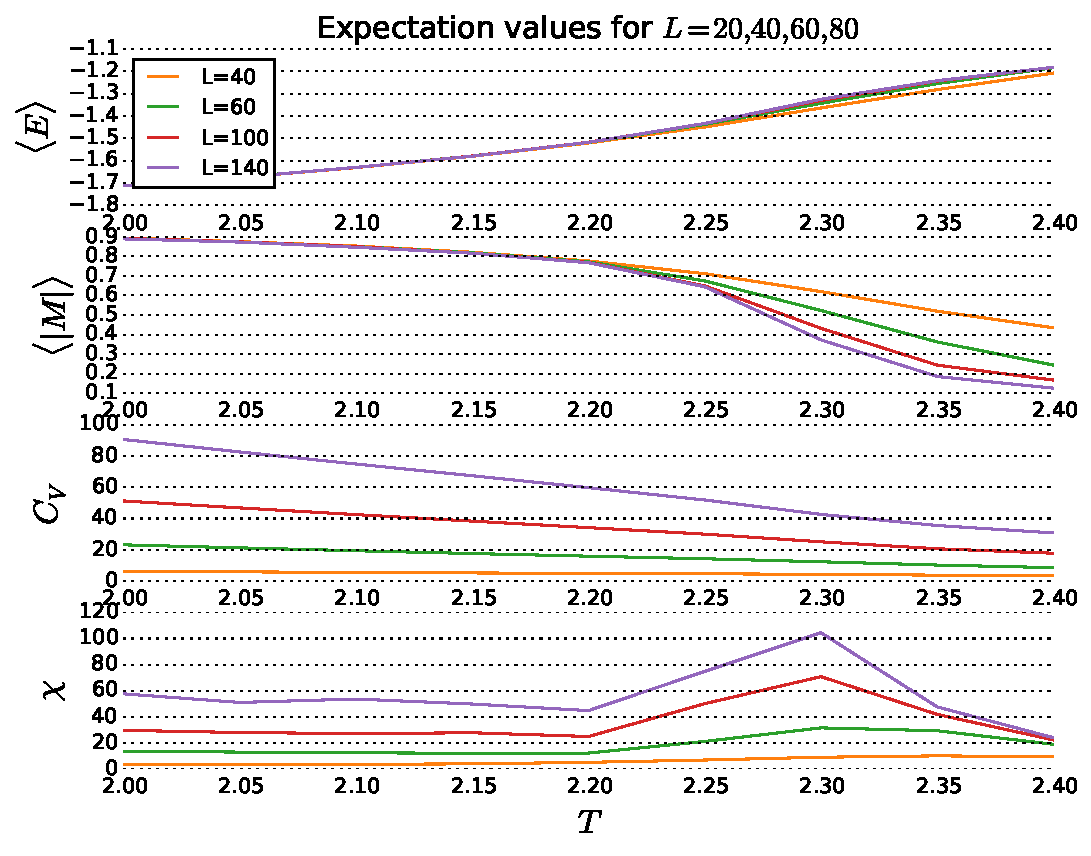
\includegraphics[width=\textwidth]{../figures/largersystems.pdf}
	\caption{The mean energy, magnetisation, specific heat and susceptibility for larger spin lattices \label{fig:largersystems}}
\end{figure}

\section{Discussion}
I have reason to believe that the graphs in figure \ref{fig:largersystems} are wrong, especially the specific heat and the susceptibility. In theory, as the size of the spin lattice approaches a very large number, one should find the Curie $T_c$ temperature, according to the following equation.
\begin{equation}
\label{eq:curie}
T_c(L\to\infty) = T_c(L)-aL^{-\frac{1}{\nu}}
\end{equation}
where the exact result gives $\nu = 1$ and $a$ is a constant.

After long hours, working through the night, in front of the computer I have regrettably been unable to uncover the problem in my program. According to Onsager \cite{onsager} the critical temperature is $kT_C/J = 2/\ln(1+\sqrt{2}) \approx 2.269$ with $\nu = 1$. This temperature would be should be clear in all the plots in figure \ref{fig:largersystems}. First, the energy plot show be splitting slightly at $T_c$. Second, the magnetisation should be falling more sharply at $T_c$, with a sharper bend for larger $L$. Third, the specific heat plot should sloping upwards before reaching a maximum at $T_c$ and then sloping downwards. Fourth, the susceptibility plot would show traits similar to the plot for specific heat, with a clear bump at $T_c$.

The plot for expected energy $\ev{E}$ and $\ev{\abs{\mathcal{M}}}$ clearly exhibits some of the these described traits, while the plot for susceptibility $\chi$ is quite close to what one would expect, but not entirely spot on. The specific heat $C_V$ on the other hand is as horrible as it could be.

I have conducted computations for spin lattices up to $L=140$ and one million Monte Carlo cycles during this study\footnote{The computations were done on the 64 core computing cluster at the Institute of Astophysics. Thanks to Trygve L. Svalheim for giving me access.}, but as I improved upon the code during the night leading up to deadline for this project I have chosen not to include the results herein as they are less accurate than the ones presented in figure \ref{fig:largersystems}. If interested, data files and a figure can be found by following the URL to github on the front page of this document.

\section{Conclusion}
In this project I employed the Ising model and the Metropolis algorithm to model a phase transition from ferromagnetic to paramagnetic material. I tried to obtain the Curie temperature, $T_c$ at which such a phase transition happens, but was only partly successful in this endeavour. Despite this I feel that I have demonstrated to a great extent how the Ising model functions and the benefit of Monto Carlo methods.

\begin{thebibliography}{9}

\bibitem{Ising} Ising, E., Beitrag zur Theorie des Ferromagnetismus,
	\emph{Z. Phys.,} 31, pp. 253-258 (1925).

\bibitem{Onsager} Onsager, L., Crystal statistics. I. A two-dimensional model with an order-disorder transition,
	\emph{Physical Review,} Series II, 65 (3-4), pp. 117-149 (1944).

\end{thebibliography}

\end{document}